\bibliographystyle{unsrt}
\chapter{Introduction au séquençage par translocation à travers un pore}
\label{intro}

\minitoc

\newpage




\section{Aspect expérimental}

\subsection{L'ADN et le séquençage}

Les bio-polymères, et notamment l'ADN (Acide DésoxyriboNucléique), sont les polymères qui constituent le vivant. Ils interviennent dans de nombreux processus clés en biologie.  L'ADN, avec l'ARN (Acide RiboNucléique) est le support de l'information génétique du vivant. \\

L'ADN, généralement contenu dans le noyau des cellules, a été pour la première fois isolé et identifié par Friedrich Miescher en 1869 à partir de globules blancs. En 1953, Francis Crick et James Watson mettent en évidence sa fameuse structure en double hélice \cite{watsoncrick}. Cette hélice est le reflet de la conformation dite double brin de l'ADN, il s'agit de l'appariement de deux chaînes dites simple brin qui sont complémentaires. Le simple brin d'ADN est une séquence de quatre monomères différents. Ces monomères, appelés nucléotides sont constitués de phosphate, de sucre et d'une des bases azotées, seul élément distinct entre nucléotides: l'adénine, la guanine (deux purines), ainsi que la cytosine et la thymine (deux pyridines). Via des liaisons hydrogènes (aussi appelée liaisons Watson-Crick dans le cas de l'ADN), les bases peuvent s'associer à leur complémentaire, adénine avec thymine et cytosine avec guanine. Les liaisons hydrogènes favorisent une forte affinité lors de l'appariement et contribuent avec les interactions orbitalaires entre cycles aromatiques des bases azotées à stabiliser cette structure hélicoïdale.

\begin{figure}[H]
\begin{center}
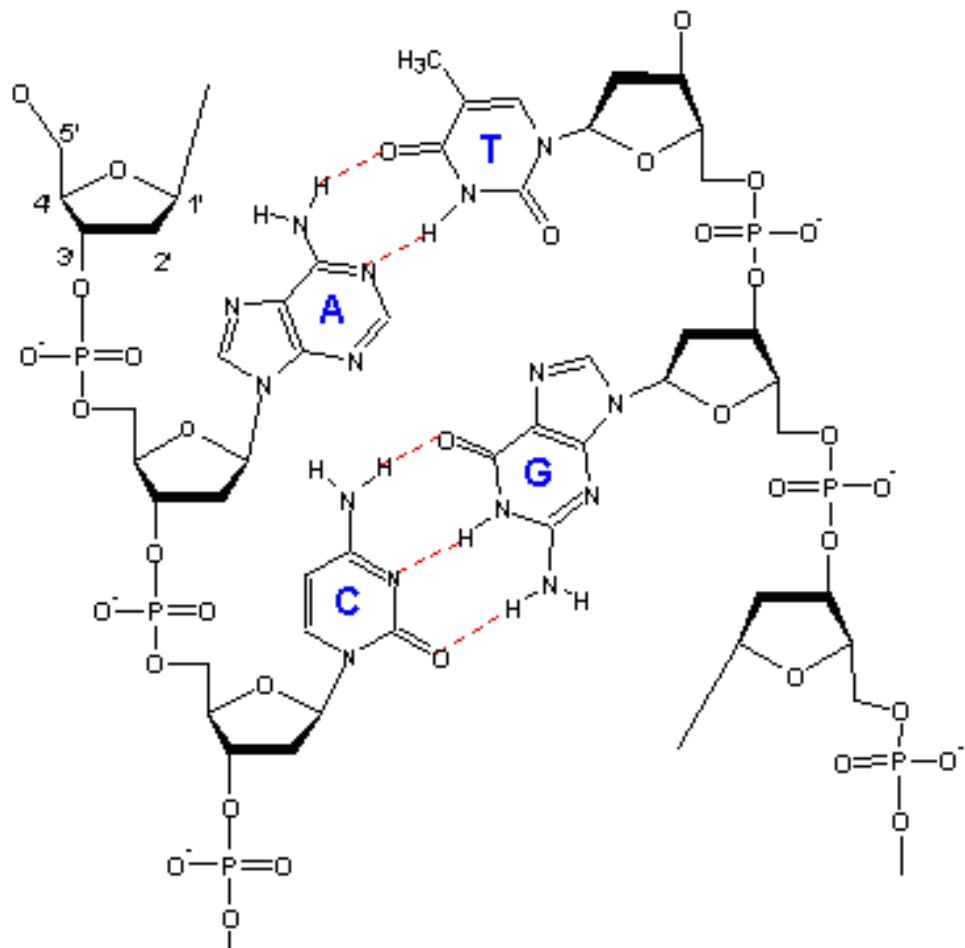
\includegraphics[width=0.63\textwidth]{adn.jpg}

\caption[Représentation de l'ADN]{Structure chimique de l'ADN. Le squelette est composé d'une succession de phosphates et de sucres liés entre eux, chacun des sucres est de plus lié à une base azotée. Les bases azotées peuvent interagir par liaisons hydrogènes et interactions orbitalaires. Les bases s'associent plus facilement avec leur complémentaire (Adénine et Thymine ou Cytosine et Guanine) permettant une certaine variété de structure: repliement d'ADN simple brins ou encore association de deux cha\^{i}nes complémentaires formant l'hélice caractéristique de l'ADN dit double brins (Image empruntée au cours de Sergei N. Smirnov \cite{adnjpg}).}
\label{adn}
\end{center}
\end{figure}

La structure chimique de l'ADN et ses intéractions (rappelées sur la figure \ref{adn}) génèrent des propriétés qui sont fortement dépendantes de la séquence. L'influence de la séquence et la compréhension du vivant passe par la capacité à séquencer l'ADN, c'est à dire déterminer l'enchaînement des nucléotides. \\

Les applications sont potentiellement nombreuses: caractérisation d'espèces vivantes \cite{Sanggaard2014}, identification de souches pathogènes pour les virus ou bactéries \cite{Janda2007}, diagnostique des maladies génétiques \cite{Saunders2012}, étude de la phylogénie \cite{Neves2011}, analyse de la résistance aux antibiotiques  \cite{Davies2010}, identification de mutations \cite{Schneeberger2009}, médecine personnalisée \cite{Hamburg2010}, identification d'individu pour la police scientifique \cite{Wilson1995}.\\


Dès la deuxième moitiée des années 70, les premières méthodes de séquençage voient le jours. Il s'agit de la méthode de Sanger \cite{Sanger1975} (voir figure \ref{sangermethod}) basée sur une synthèse enzymatique sélective (inspirée des travaux de Wu, R Padmanabhan et al \cite{WU1972}, qui déterminèrent la première séquence de 24 paires de bases) et de la méthode Maxam et Gilbert \cite{Maxam1977} basée sur une dégradation chimique sélective. Gilbert et Sanger obtiennent tous deux le prix Nobel de médecine en 1980 pour leurs méthodes. En 1977, grâce à sa méthode, Sanger parvient à séquencer le premier génome complet, il s'agit du bactériophage $\Phi$X174 \cite{Sanger1977}.\\

\begin{figure}[H]
\begin{center}
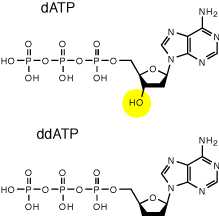
\includegraphics[width=0.5\textwidth]{ddatp.png}\hspace{1.3cm} 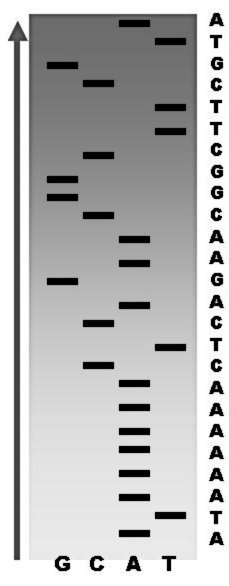
\includegraphics[width=0.21\textwidth]{gelelectrophoresis.jpg}
\vspace{0.5cm}

\caption[Séquencer par la méthode de Sanger]{Le séquençage par la méthode de Sanger : Le brin d'ADN à séquencer est répliqué parallélement dans quatres milieux différents contenant chacun les quatre désoxyribonucléotides (dATP, dCTP, dGTP, dTTP). Chacun des milieux présente en plus une faible quantité de l'un des didésoxynucléotides (ddATP, ddCTP, ddGTP ou ddTTP), qui une fois incorporé dans la cha\^{i}ne empêche toute croissance supplémentaire (image de gauche). Chacun des quatre milieux présente alors des cha\^{i}nes de tailles variées terminant toutes par un même nucléotide. Les milieux sont alors analysés par électrophorèse sur gel, ce qui va trier les cha\^{i}nes par taille. On peut alors remonter à la séquence par lecture directe sur le gel (image de droite).}
\label{sangermethod}
\end{center}
\end{figure}



 
 La méthode de Sanger est rapidement préférée à celle de Maxam-Gilbert car elle nécessite moins de composés chimiques toxiques et de marqueurs radioactifs. Elle a été utilisée du début des années 80 jusqu'à la moitié des années 2000 avec principalement des avancées techniques:  marquage fluorescent \cite{Prober1987}, électrophorèse capillaire \cite{Swerdlow1991} ou encore automatisation des procédures \cite{Hunkapiller1991}.\\
 
  Afin de séquencer de longs génomes, les nouvelles techniques utilisent de la méthode dite shotgun, qui reconstruit un génome complet à partir de fragments de séquences moins couteux et plus simples à séquencer, élaborée par R. Staden \cite{Staden1979} (voir figure \ref{shotgun}).
 


\begin{figure}[H]
\begin{center}
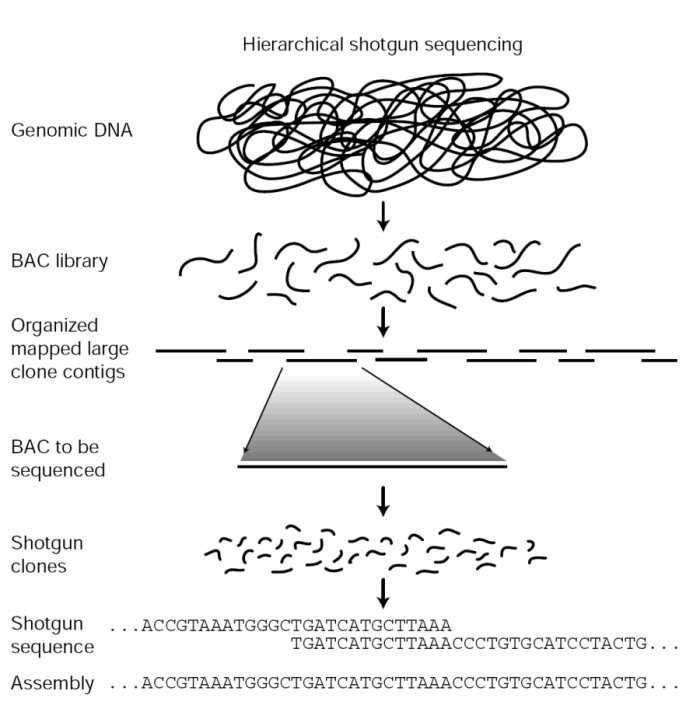
\includegraphics[width=0.8\textwidth]{shotgun.jpeg}
\vspace{0.5cm}

\caption[Méthode Shotgun]{Schéma de principe de la méthode shotgun (emprunt à la review de Eric S. Lander et al.\cite{Lander2001}). Le brin étudié est d'abord copié de nombreuses fois par PCR. Les brins sont ensuites fragmentés pour créer une banque de séquences aléatoires plus courtes (et moins compliquées à séquencer) qui sont également marquées. Ces fragments subissent à nouveau une PCR et forment de nombreux clones rassemblés chacun dans une colonie (ou polonie, contraction de PCR et colonie, voir figure \ref{pcr}). Chaque colonie est alors séquencée. De lourds traitements informatiques sont enfin employés pour reconstituer la séquence d'origine à partir des parties de génomes qui se chevauchent entre séquences.}
\label{shotgun}
\end{center}
\end{figure}

 En plus de nécessiter une librairie de base, ces techniques impliquent une amplification du signal ADN de départ par PCR (Polymerase Chain Reaction) \cite{Saiki1985}, de lourd traitements algorithmiques et sont sujettes à des erreurs notamment en ce qui concerne les parties de séquences redondantes dont certaines peuvent être ommises. Deux types de PCR seront successivement utilisées. La PCR en émulsion \cite{Williams2006}, puis la PCR directement sur lames de microscopes \cite{Shendure2005}. La figure \ref{pcr} présente le concept de PCR et ces deux exemples. Cette première génération de séquençage a permis en 2001 le premier séquençage complet du génome humain \cite{Lander2001,Venter2001}.





 \begin{figure}[H]
\begin{center}
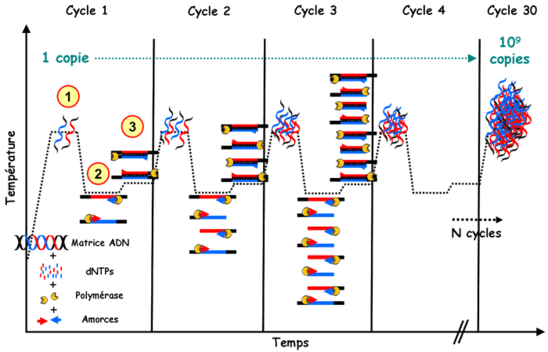
\includegraphics[width=0.9\textwidth]{pcr.png}

\vspace{0.5cm}

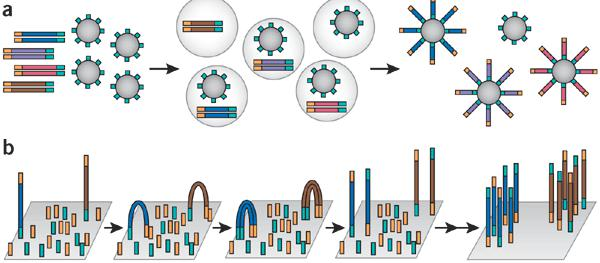
\includegraphics[width=0.9\textwidth]{bridgepcr.jpg}
\vspace{0.5cm}

\caption[PCR]{En haut, schéma de principe d'une PCR (Polymerase Chain Reaction), emprunt au site de l'université de strasbourg \cite{pcrjpg}. En bas, illustration de la review de Shendure \cite{Shendure2008}. a/ Une PCR réalisée en émulsion, les cycles successifs sont réalisés au sein d'une goute en suspension. b/ Une PCR sur lame de microscope, la multiplication de l'ADN a lieu sur une zone restreinte grace à un système de liaison covalentes avec les amorces de la réaction. Chaque goutte en suspension ou chaque zone sur la lame de microscope est appelée colonie d'ADN (ou polonie, contraction de PCR et colonie). Une polonie contient un unique fragment de la banque d'ADN. Les différents appareils commerciaux se distingueront dans un premier temps uniquement dans la façon d'effectuer la PCR et/ou de séquencer ces polonies.}
\label{pcr}
\end{center}
\end{figure}


Brevetées dans les années 90 \cite{tsien1991dna,farinelli1998method}, les méthodes précédemment décrites vont être utilisées dans des appareils de séquençage commerciaux, ce qui va populariser l'utilisation du séquençage \cite{Schuster2007}. Ces appareils se distinguent principalement par les moyens utilisés afin de séquencer la banque d'ADN obtenue dans le cadre de la méthode shotgun. Le premier appareil de cette génération, le MPSS ( Massively parallel signature sequencing \cite{Brenner2000}) voit le jour en 2000. Il repose sur une méthode tellement complexe qu'aucun appareil n'a été fourni à des laboratoires indépendants, les séquençages ayant lieux dans les locaux de la companie Lynx Therapeutics. D'autres appareils sont développés en parallèle. En 1996 le pyrosequencing \cite{Ronaghi1996}, séquençage qui repose sur la détection de l'activité de l'ADN polymérase par un pyrophosphate voit le jour. Ce procédé sera utilisé par un appareil commercial de la société 454 Life Sciences en 2005 \cite{Margulies2005}. Life Technologies avec le séquençage SOLiD \cite{mckernan2007reagents,Cloonan2008} (Sequencing by Oligonucleotide Ligation and Detection) commercialise son appareil en 2008. Il s'agit de séquençage par ligation, ce dernier repose sur une identification de la séquence par la forte spécificité de l'ADN ligase, qui va lier à l'aide d'une séquence de référence, un brin complémentaire, préalablement marqué, à la séquence inconnue. La partie liée est caractéristique de deux bases successives. Quatre flurophores différents sont utilisés et chacun des fluorophores est donc caractéristique de quatre doublets de bases ( il y en a $2^{4}=16$ différents répartis sur quatre fluorophores). Des lectures successives en décallant les ligation d'une base permettent de déduire la séquence. Ce système a vu le jour dans un premier temps avec une PCR en émulsion puis une version utilisant une PCR sur support solide a été dévelloppée. Cette technique est efficace mais présente cependant des erreurs lors de la lecture de séquences palindromiques \cite{Huang2012}. La société Illumina en 2008 \cite{Bentley2008} sort le premier appareil basé sur une PCR sur support solide, Le séquençage est réalisé par la lecture de fluorophores lors de l'incoporation de bases modifiées au cours de la PCR. Le marquage est retiré à chaque étape de lecture. Life Technologies utilise quand a elle aussi le séquençage par semi conducteurs pour détecter les ions hydrogènes relachés lors de la polymérisation de l'ADN (Ion semiconductor sequencing) \cite{Rusk2010}, cette méthode est efficace, mais rencontre des  problèmes avec les répétitions d'homopolymers \cite{Rusk2010}. 

\begin{figure}[H]
\begin{center}
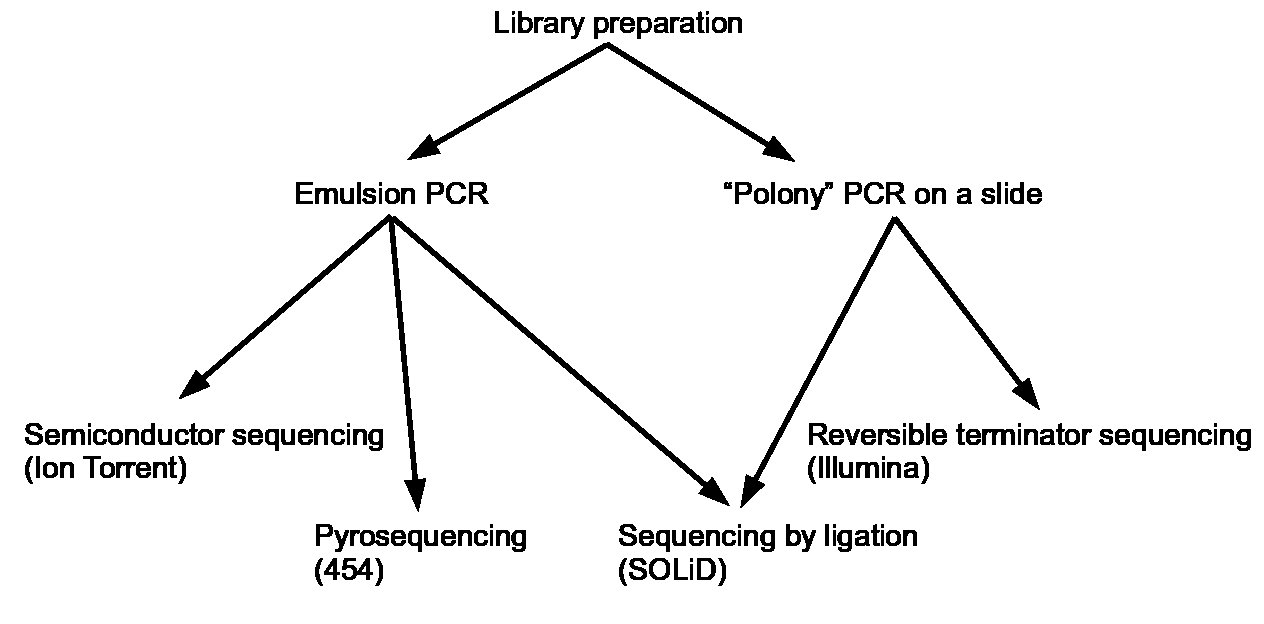
\includegraphics[width=0.8\textwidth]{ngsprinciple.jpg}
\vspace{0.5cm}

\caption[Principe du "next gen sequencing"]{Schéma récapitulatif du fonctionnement des premiers appareils de séquençage de nouvelle génération \cite{ngsprinciplejpg}.}
\label{ngsprinciple}
\end{center}
\end{figure}

Comme nous l'avons vu, ces procédés nécessitent une PCR pour amplifier le signal ADN de départ. Cette étape est source d' erreurs, en effet la PCR peut être biaisée et peut générer des artefacts \cite{Acinas2005}.



Deux autres techniques de lecture sans amplification sont développées, DNA nanoball sequencing \cite{Porreca2010} et Heliscope single molecule sequencing \cite{pmid20890904}, mais restent peu utilisées car elles ne sont utilisables que sur des fragments d'ADN très courts. Une approche originale est également commercialisée, il s'agit du séquençage en temps réel d'une molécule unique (Single molecule real time sequencing), un marquage fluorescent est détecté lors de la création du brin complémentaire lors de la copie de l'ADN \cite{Eid2009}. Cependant plusieurs lectures sont nécessaire pour obtenir une précision suffisante \cite{Chin2013}. Ces derniers appareils sont précurseurs de la troisième génération de séquençage en manipulant des molécules uniques.



Certains de ces appareils sont comparés dans le tableau récapitulatif suivant, créé à partir des résultats comparés entre différents appareils \cite{Quail2012,Liu2012}. \textcolor{red}{tableau a faire}

\begin{figure}[H]
\begin{center}
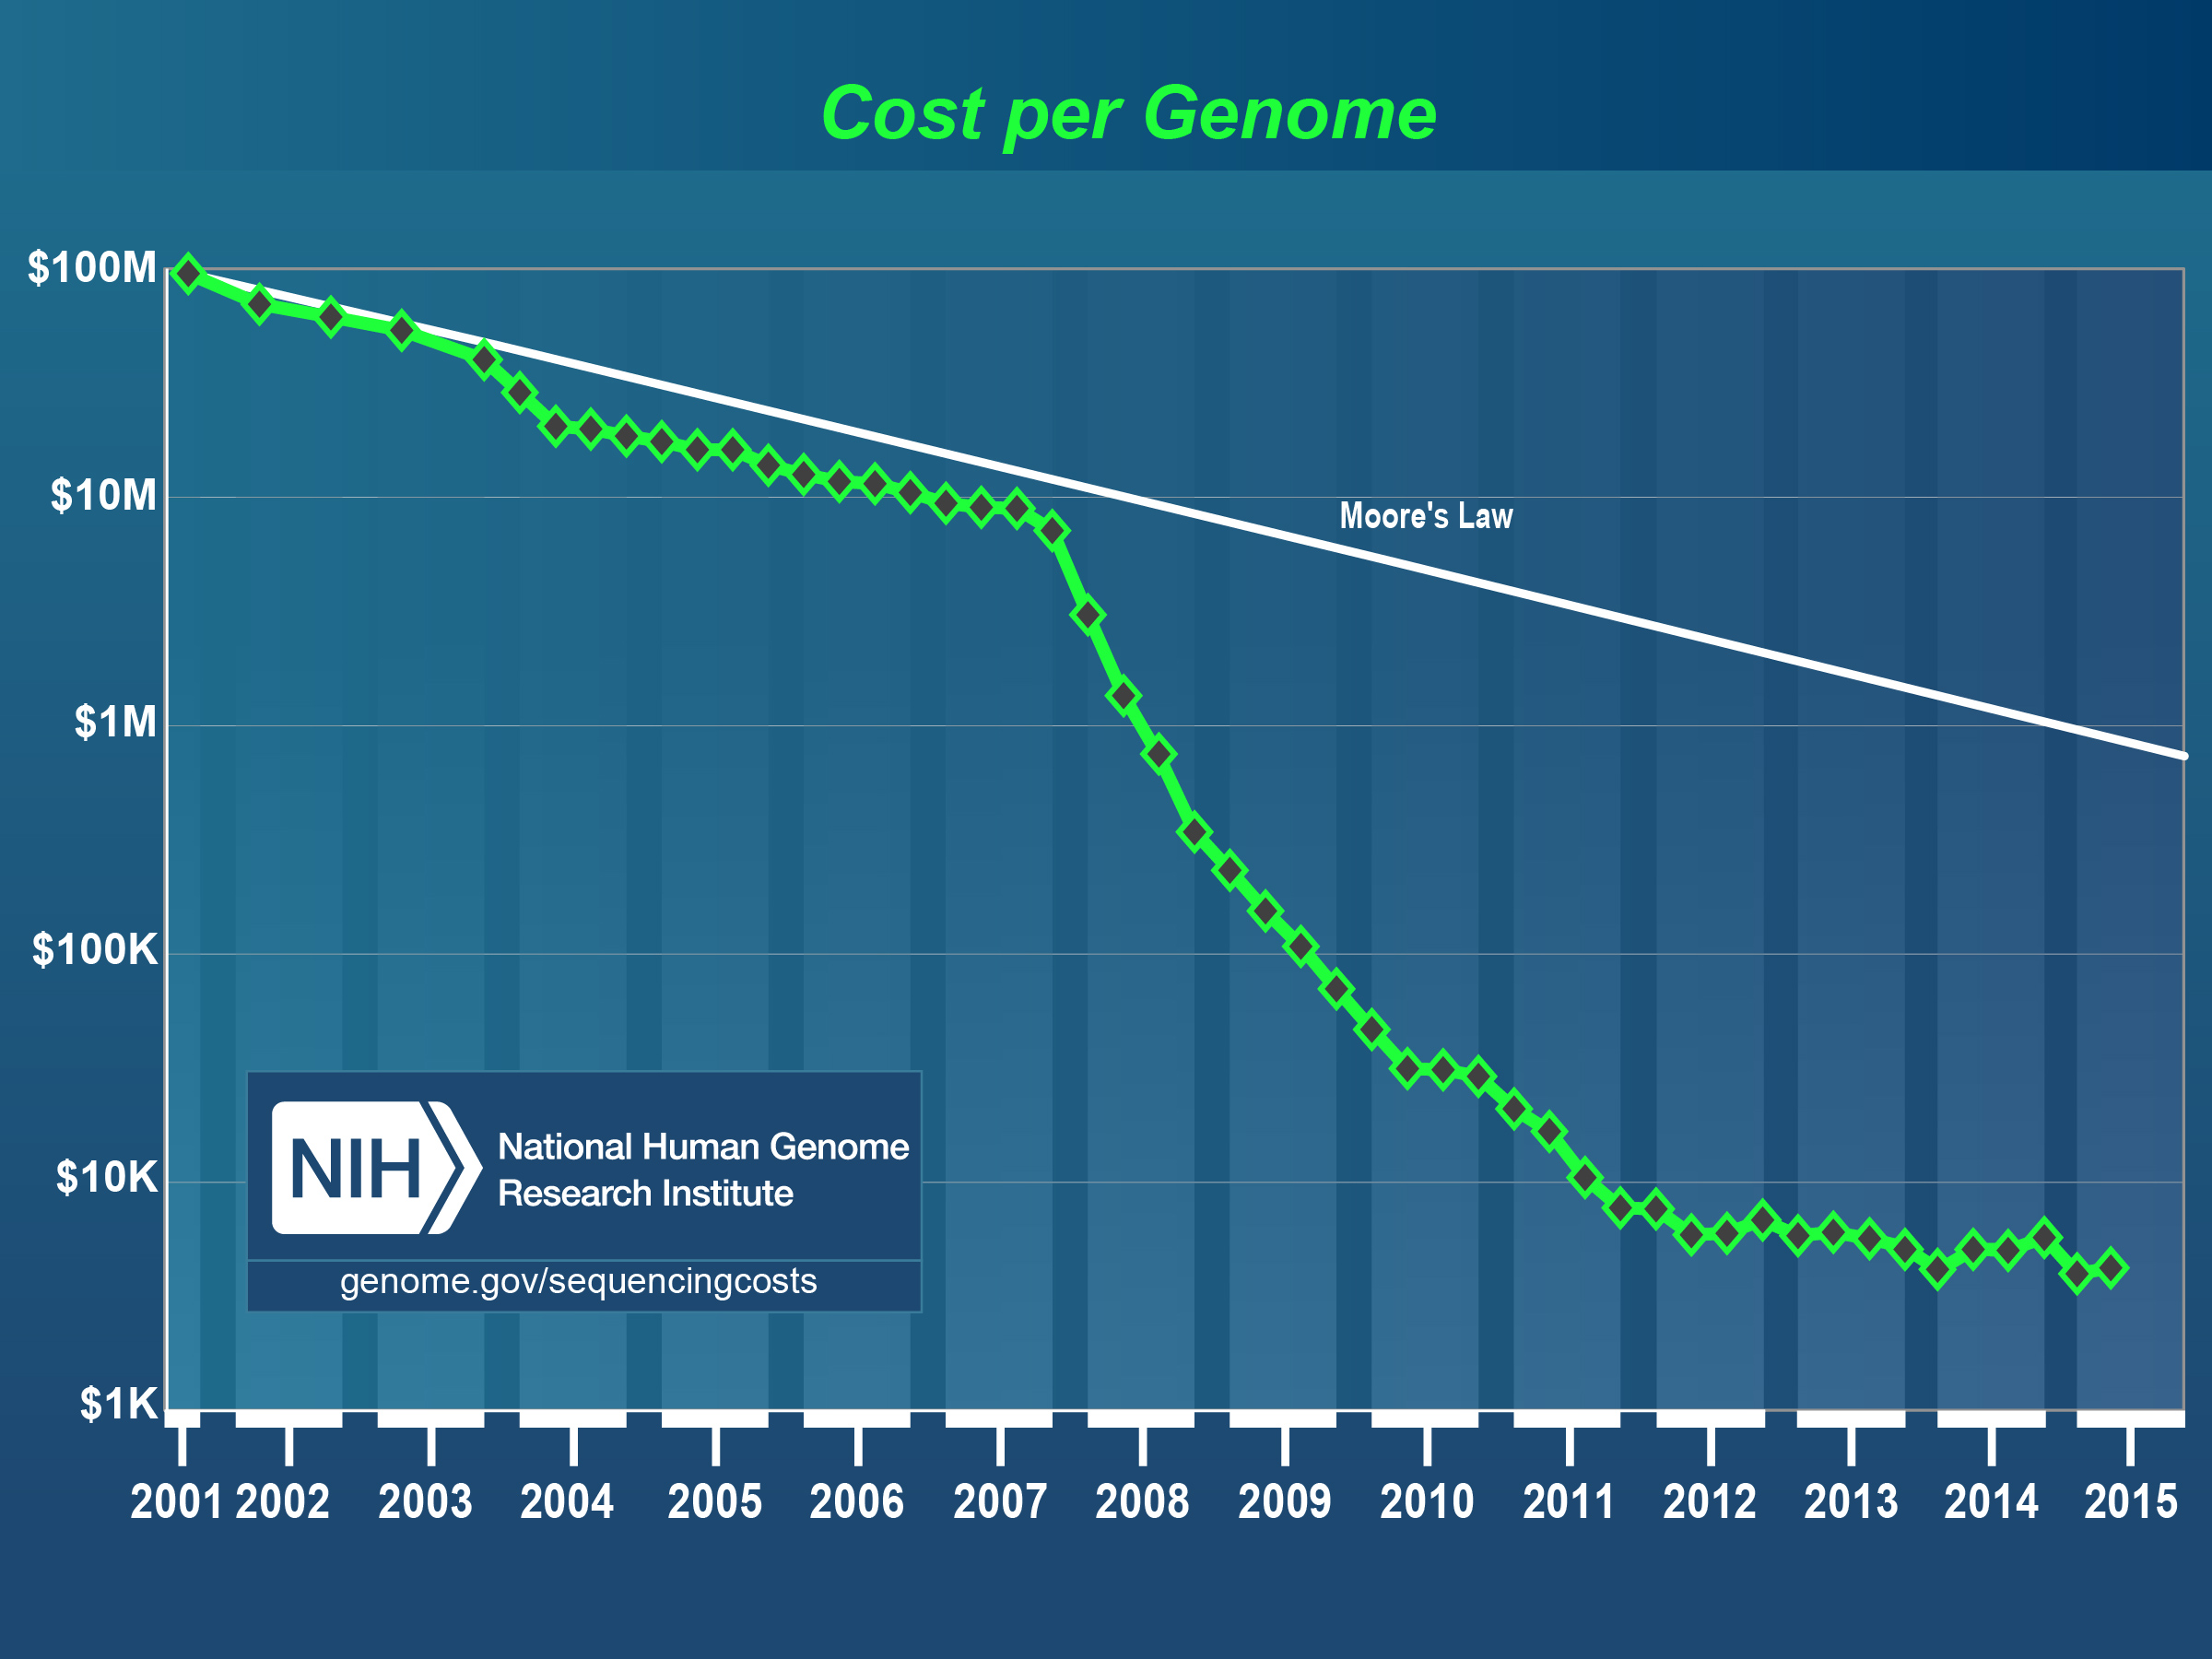
\includegraphics[width=0.7\textwidth]{cost_genome.jpg}

\caption[Coût du séquençage]{Evolution du coût du séquençage d'un génome complet selon le NIH. On observe au départ une diminution normale du coût suivant une loi de Moore. L'arrivée des premiers appareils commerciaux de séquençage de nouvelle génération se traduit par une rupture de pente très nette en 2007. Aujourd'hui, un plateau au dessus de l'objectif des 1000 USD pour un génome complet est atteint, d'où la nécessité de développer des méthodes dites de troisième génération.}
\label{seqcost}
\end{center}
\end{figure}

La figure \ref{seqcost} présente l'évolution du coût du séquençage d'un génome complet. Nous sommes toujours au dessus de l'objectif de 1000 USD \cite{Mardis2006}.

Tous ces appareils commerciaux  ont fait leurs preuves mais leur utilisation demeure trop coûteuse pour envisager leur usage à grande échelle. Une troisième génération de technique de séquençage est aujourd'hui envisagée.\\

Voici une liste de pistes envisagées pour les appareils de séquençage de troisième génération:

\begin{itemize}


\item Le séquençage par hybridation \cite{Zhang2003}. Ce procédé permet de reconnaitre des séquences types par leur hybridation avec des bio-puces à ADN ( de courtes séquences), cela nécessite un marquage fluorescent ainsi qu'un nombre important de produits chimiques et d'ADN de base.

\item L'utilisation de la spectroscopie de masse \cite{Edwards2005}. Basée sur la différence de masse entre les nucléotides, cette méthodes semble être adaptées à la détection de substitution de bases dans différents gênes, mais pas pour séquencer des génomes de novo (dans leur intégralité). Elle s'avère utile cependant pour la médecine légale \cite{Howard2013}. 

\item La mise au point de techniques de microscopie électronique \cite{Bell2012}. Ces techniques sont complexes car elles nécessitent une modification des bases de l'ADN pour incorporer des atomes au numéro atomique élevé, afin d'obtenir un contraste suffisant.

\item La manipulation de bio-molécules avec pinces optiques, magnétiques ou AFM \cite{Pareek2011,Ding2012}.

\item La mesure du courant obtenu par effet tunnel lors du passage de l'ADN dans un canal microfluidique \cite{Ohshiro2012,DiVentra2013}.

\item \textbf{Le séquençage par nanopore.}


\end{itemize}


C'est cette dernière possibilité que nous explorons. Un appareil commercial de la société Oxford Nanopores Technologies a vu le jours au cours de la thèse \cite{Mikheyev2014,Goodwin2015,Urban2015} et commence à être utilisé. Il est décrit dans le sous-chapitre suivant.


\textcolor{red}{à regarder dans reviewngs2012n2 \cite{Liu2012}.}

\subsection{Utilisation de nanopores}

Le séquençage par nanopore a potentiellement de nombreux avantages sur les systèmes commerciaux déjà existants. En effet, cette technique laisse envisager la lecture de longues séquences (supérieurs à 5000 paires de bases) à vitesse élevée (1 paire de base par nanoseconde) \cite{Timp2010,Branton2008}. Aucun marquage chimique n'est nécessaire, l'utilisation d'enzymes est moindre et le signal ADN n'a pas besoin d'être amplifié (pas de PCR).

Exposons dans un premier temps les concepts de bases et définitions du séquençage par nanopore. On envisage de séquencer la séquence ADN au cours de sa translocation. La translocation, c'est le passage d'un polymère d'un coté, appelé cis, d'une membrane à l'autre, appelé trans, à travers un pore (voir figure \ref{translocbase}). Cette translocation peut être naturelle (non biaisée) ou pilotée par une force (biaisée). La translocation est un phénomène biologique fréquent, c'est le cas par exemple lorsqu'un virus infecte une cellule en y translocant son ADN.

\begin{figure}[H]
\begin{center}
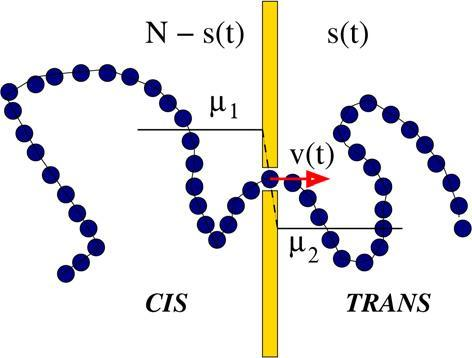
\includegraphics[width=0.44\textwidth]{translocation.jpg} 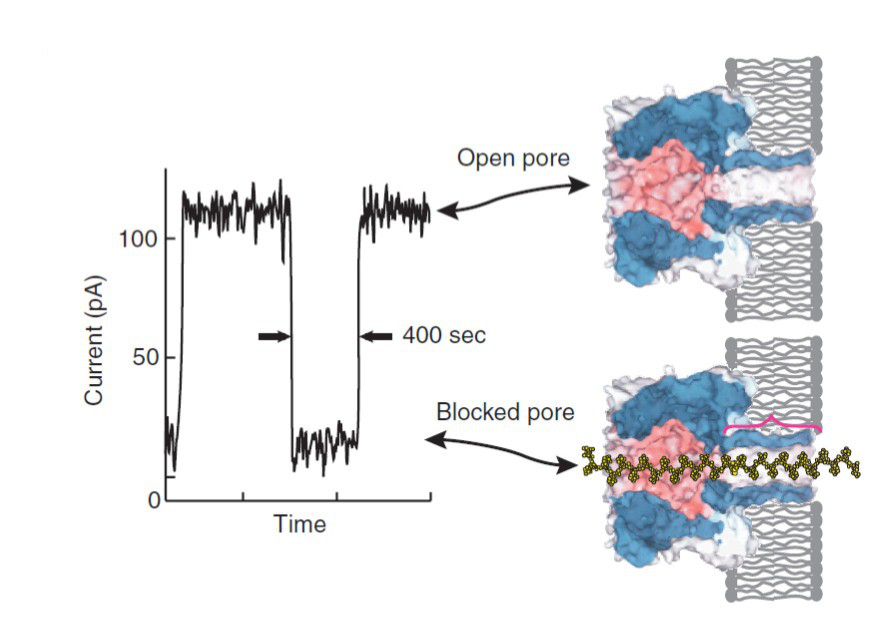
\includegraphics[width=0.55\textwidth]{translocissues.jpg}

\caption[translocation et courant de blocage]{Translocation d'un polymère. A gauche: Illustration de la translocation biaisée d'un polymère par l'application d'une différence de potentiel chimique empruntée à la review de A. Milchev \cite{Milchev2011}. A droite: Translocation d'ADN à travers un biopore et mesure du courant de translocation illustrés par Branton et al. \cite{Branton2008}.}
\label{translocbase}
\end{center}
\end{figure}

Au cours de la translocation de l'ADN, on espère pouvoir séquencer en mesurant le courant de translocation. Le principe est simple, au cours de la translocation, l'occupation du pore entraine une modification de sa résistance électrique, modification caractéristique de l'entité occupant ce pore. On peut alors espérer déterminer la nature de l'occupant du pore (typiquement la séquence pour l'ADN) en mesurant le courant ionique de blocage du pore (voir figure \ref{translocbase}). On dispose déjà de certaines applications de ce procédé, notamment pour le comptage de polymers \cite{Bezrukov1994}, la détection d'ADN et ARN \cite{Kasianowicz1996} ou encore la discrimination de certains polynucleotides \cite{Akeson1999,Meller2000,Ashkenasy2005}. Cette technique bien que prometteuse admet des limites de résolution spatiales et temporelles qui font qu'elle ne permettra pas de séquencer l'ADN \cite{Branton2008}. Nous expliquerons ces limites en décrivant les différent types de nanopores disponibles ainsi que les techniques alternatives qui s'inspirent de la mesure du courant ionique de blocage, dans le paragraphe suivant.

\textcolor{red}{c'est démontré que courant ionique classique ne peut pas distinguer donc courant transverse ou fonctionnalisation. j en parlerais après description des différents nanopores.}

\subsubsection{Les différents nanopores}


Historiquement, les premier nanopores utililsés sont ceux fournis par la nature. On peut employer la protéine F située sur la membra ne extérieurs de Escherichia Coli \cite{Danelon2006,Chimerel2008})
ou encore l'$\alpha$-hémolysine du Staphylocoque doré \cite{Bhakdi01121991}. Ce dernier est très utilisé car il est disponible commercialement, d'une reproductivité parfaite et est susceptible d'être employé avec de l'ingénierie génétique pour modifier certaines propriétés (blocage au passage d'ADN par exemple \cite{Howorka2001}). Il s'agit d'ailleurs du biopore utilisé par Kasianowicz et al. pour effectuer en 1995 la première translocation d'ADN \cite{Kasianowicz1996}.


\begin{figure}[H]
\begin{center}
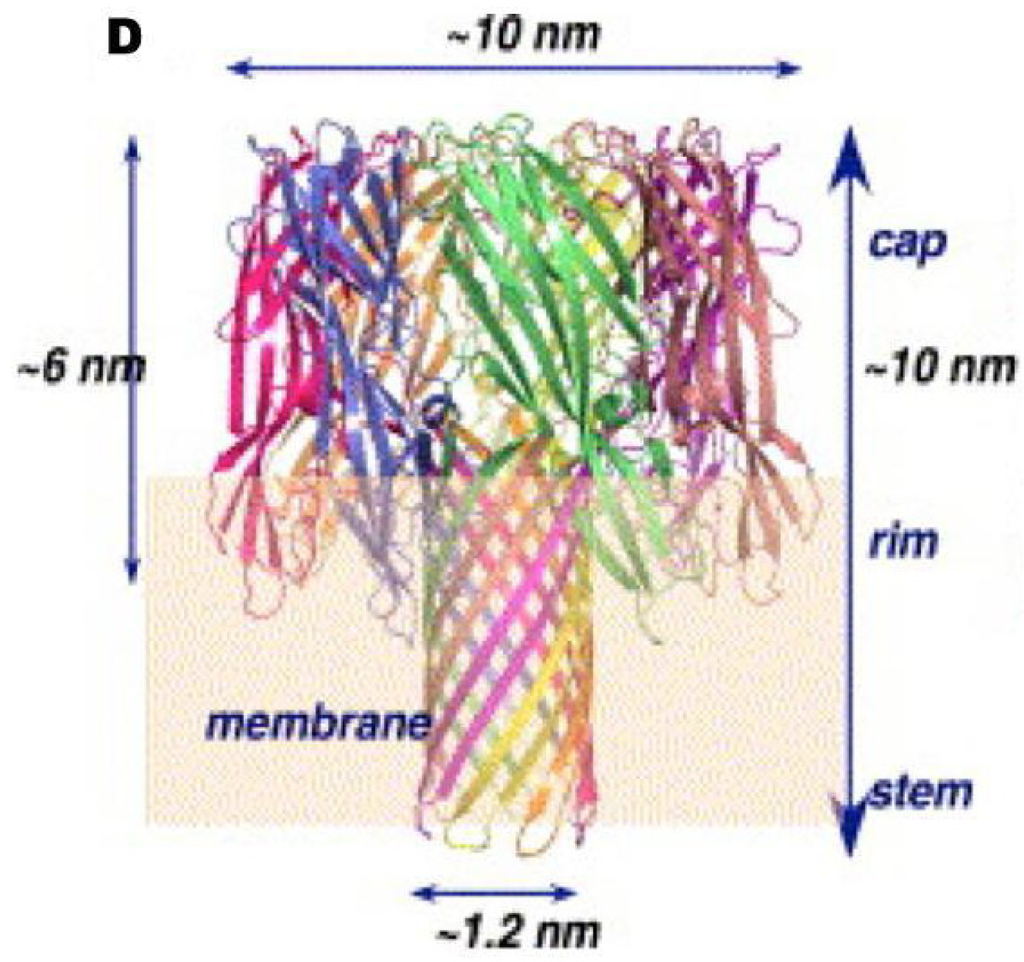
\includegraphics[width=0.54\textwidth]{bioporetoxine.png}
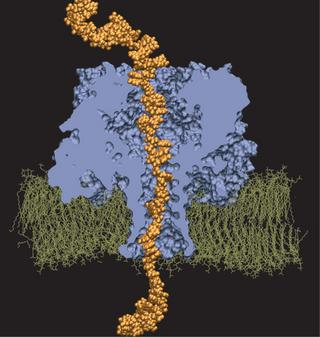
\includegraphics[width=0.44\textwidth]{biopore2.jpg}

\caption[Biopores]{Les biopores ont été les premiers pores utilisés à des fin d'étude ou d'emploi des phénomènes de translocation. A gauche, model du pore heptameric de B. cereus \cite{Ramarao2013}. A droite, simulation de translocation d'ADN à travers un biopore ($\alpha$-hémolysine) \cite{Aksimentiev2010}.}
\label{biopore}
\end{center}
\end{figure}

Ces biopores ont prouvé leur efficacité pour la translocation d'ADN et ARN simples brins ou encore pour des protéines dépliées \cite{Movileanu2005}. Ils demeurent trop étroit pour les formats double brin car leur diamètre n'est pas réglable. La nature fourni des outils efficaces, car avec la l'utilisation en complément de protéines chaperonnes, il est possible d'empécher l'inversion de la translocation \cite{DeLosRios2006} (phénomène qui inspira la fonctionalisation des autres types de pores dont nous allons parler par la suite). La figure \ref{bioporepossib} présente un inventaire succins des possibilitées offertes par les biopores. Dans une optique de séquençage, ils sont trop épais pour permettre de discriminer les séquences en cours de translocation.

\begin{figure}[h!]
\begin{center}
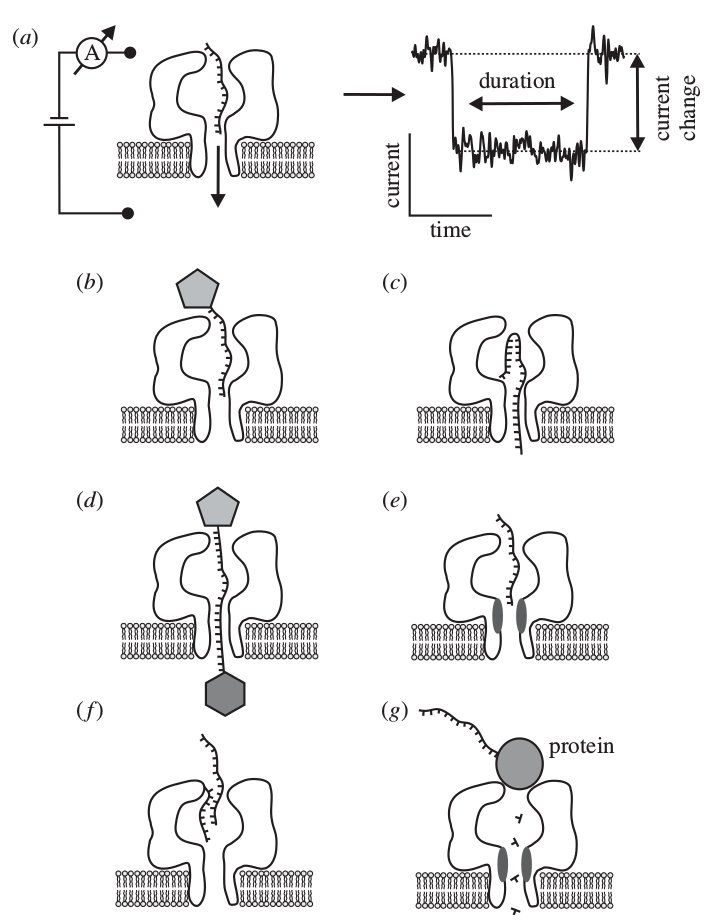
\includegraphics[width=0.85\textwidth]{bionanopore.jpg}


\caption[Manipulation sur biopores]{Différentes manipulation possibles avec les biopores (emprunt à la review de U. F. Keyser \cite{keyser}). a/ Mesure du courant ionique de translocation. b/ Une protéine plus large que le pore fixée sur l'ADN permet d'imposer le sens de la translocation. c/ Un brin replié sur lui même peut stopper la translocation. d/ Attacher une protéine à chaque extrémité de l'ADN peut conduire à une translocation à durée infinie. e/ La modification génétique du pore peut affecter la translocation. f/ Le pore peut être fonctionnalisé avec de l'ADN complémentaire d'une séquence à détecter. g/ Une endonucléase peut être combinée au nanopore pour réaliser une translocation base par base.}
\label{bioporepossib}
\end{center}
\end{figure}



Les limites des biopores ont poussé les chercheurs à développer leur propres pores. En 2001 le premier nanopore artificiel est créé \cite{Li2001}. Un faisceau concentré d'ions ou d'électrons peut être utilisé pour creuser un pore dans une membrane de matériaux variés\cite{Wanunu2010}.

\begin{figure}[h!]
\begin{center}
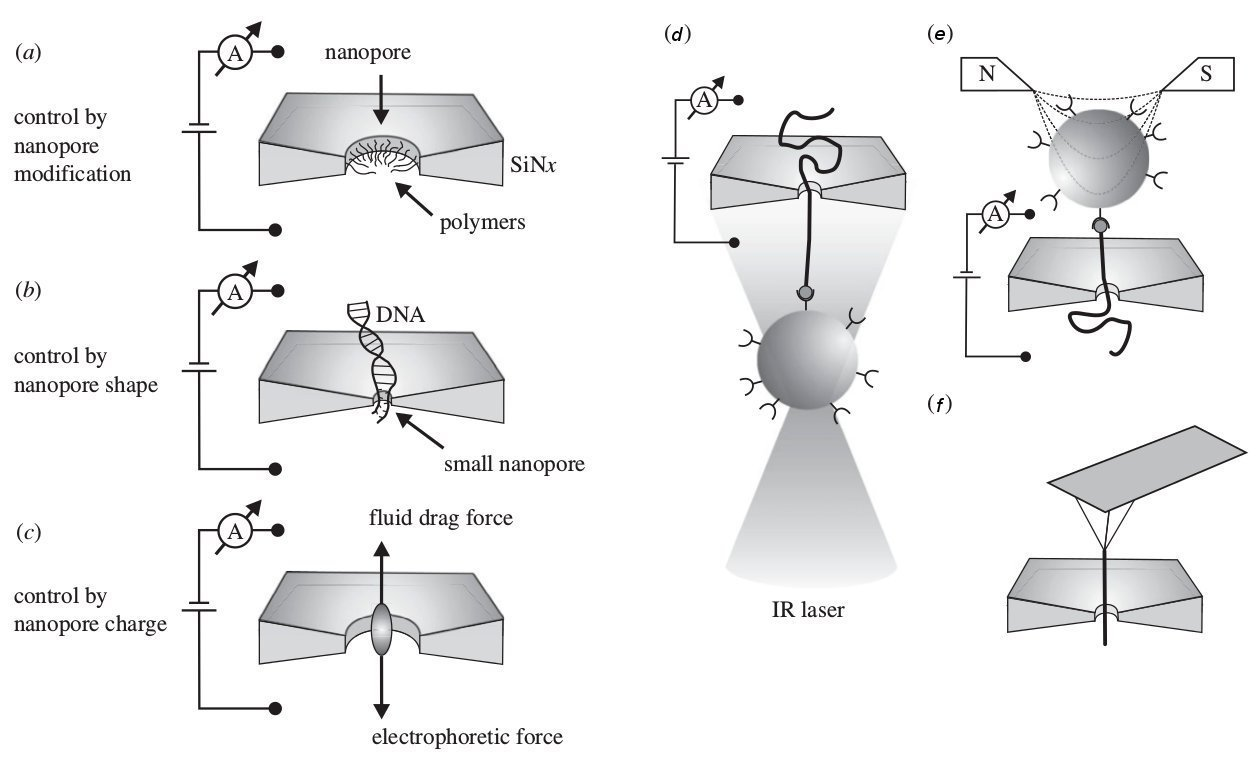
\includegraphics[width=1.0\textwidth]{solidstatenanopore.jpg}


\caption[Pores artificiels et manipulations]{A gauche, différentes modifications possibles avec les pores artificiels, à droite, les différents controles mécaniques possibles pour la translocation (emprunt à la review de U. F. Keyser \cite{keyser}). a/ Fonctionalisation du nanopore. b/ Gestion de la taille du nanopore. c/ Contrôle de la charge du pore (pouvant ralentir la translocation en générant une résistance hydrodynamique plus importante). d/ Utilisation de pinces optiques. e/ Utilisation de pinces magnétiques. f/ ADN accroché à une pointe d'AFM. }
\label{solidstateporepossib}
\end{center}
\end{figure}


L'arrivée des nanopores artificiels a permis de travailler dans des conditions controlées. La posibilité de choisir le diamètre et les propriété du pore s'accompagne du développement de techniques de manipulation pour forcer la translocation (voir la Figure \ref{solidstateporepossib}).




hybrid (alpha machin greffé dans un solid state nanopore \cite{Hall2010})


\begin{figure}[h!]
\begin{center}
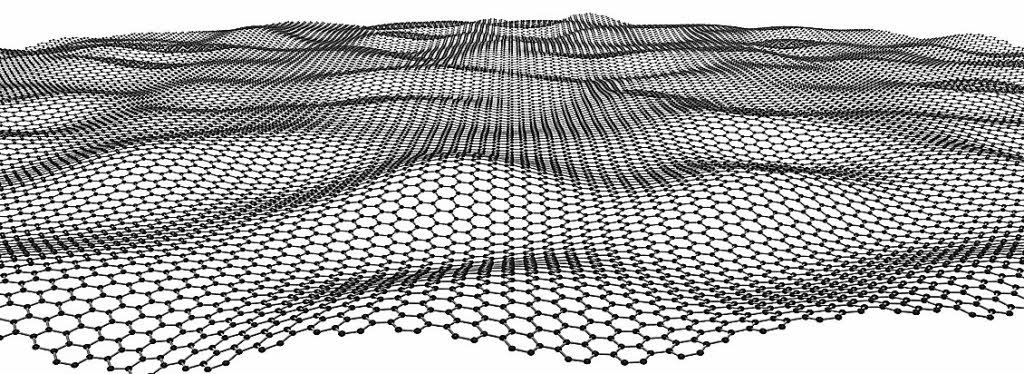
\includegraphics[width=1.0\textwidth]{vib.jpg}


\caption[Vibration et déformation d'une mono-couche de graphène]{Illustration de Jannik C. Meyer, qui a travaillé sur les membranes de graphènes \cite{Meyer2007}. La faible épaisseur des membranes monoatomiques entraine une forte influence des vibrations, déformations et de la flexibilité.}
\label{membvib}
\end{center}
\end{figure}

arrivée du graphène et autres cristaux bidim fins (Electrochemical Reaction in Single Layer MoS2: Nanopores Opened Atom by Atom \cite{Feng2015}).








a garder en memoire : ralentissement de la transloc avec nanopore plus petit que la double hélice (à citer dans papier et dans these quand transloc ralentie par pore étroit)\cite{Mirsaidov2010}

mesure coefficient de diffusion de l ADN \cite{Smith1996}

enveloppe dna en traction \cite{Wirtz1995}



\subsection{La translocation de polymères}



